\documentclass{article}
\usepackage{ctex}
\usepackage{graphicx} % Required for inserting images
\usepackage{subfig}
\usepackage{float}
\usepackage[colorlinks=true, linkcolor=blue, urlcolor=red, citecolor=red]{hyperref} % 超链接支持
\title{第三章函数拟合实验总结}
\author{樊建琦}
\date{October 2024}

\begin{document}

\maketitle

\section{Introduction}
第二章、第三章的内容集中讨论函数逼近的问题,插值亦或拟合,或理论或应用,总归落在了拟合二字。实验三系统性的从随机采样到切比雪夫采样;从插值函数到拟合函数,最终得到$P^{*}(x),P^{*}(x) \in H_{n}$. 为了评价拟合优劣,我们用matlab在画布中描出准确值$(gt)$与预测值$(pred)$,用二者的平均误差和整体重合程度评价拟合程度。但最小二乘中二范数对噪声有着本源的低抗性,所以我们在每个实验方法后都添加了扰动环节,考察引入扰动后,偏移程度是否能被接受。
\section{Newton Interpolation}
方案一选取随机采样点,方案二选取切比雪夫多项式零点作为采样点,采用牛顿插值法进行插值,画出插值函数和原函数曲线,对比分析插值结果的龙格现象差异。
\begin{figure}
    \centering
    \includegraphics[width=0.8\textwidth]{prob1/fig12.png}
    \label{fig:cheb_random}
\end{figure}
\hyperref[fig:cheb_random]{Fig.1-1,1-2 }分别是采样方式为切比雪夫零点、随机取点,可以看到,这两种采样方式得到的误差都相对较小,切比雪夫零点的误差小是因为它把$R_n(x) = \frac{f^{(n+1)}(\xi)}{(n+1)!} \prod_{i=0}^{n} (x - x_i)$中的$\prod_{i=0}^{n} (x - x_i)$取到了最小。
但是均匀采样如\hyperref[fig:uniform]{Fig.1-3}所示,误差极大,一方面是为了迎合多变的目标函数,多项式最高次数必须有一定的规模,因此导致的边界龙格效应,另一方面是因为由于均匀分布的采样点在区间边界附近的密度较低,导致误差项在区间边界附近较大,从而出现龙格现象。 
\begin{figure}[H]
    \centering
    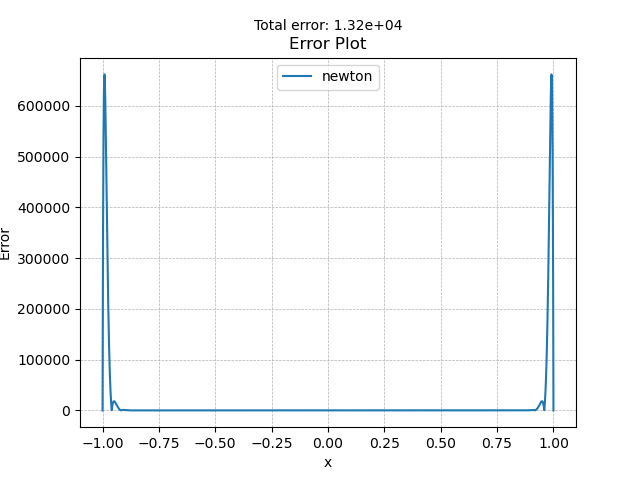
\includegraphics[width=0.8 \textwidth]{prob1/sub_error_uniform.png}
    \caption{Caption}
    \label{fig:uniform}
\end{figure}
三种方法对比图如\hyperref[fig:contrast]{Fig.1-3 }所示,切比雪夫与随机取样显然优于均匀采样,且龙格效应被大幅度抑制。
\begin{figure}[H]
    \centering
    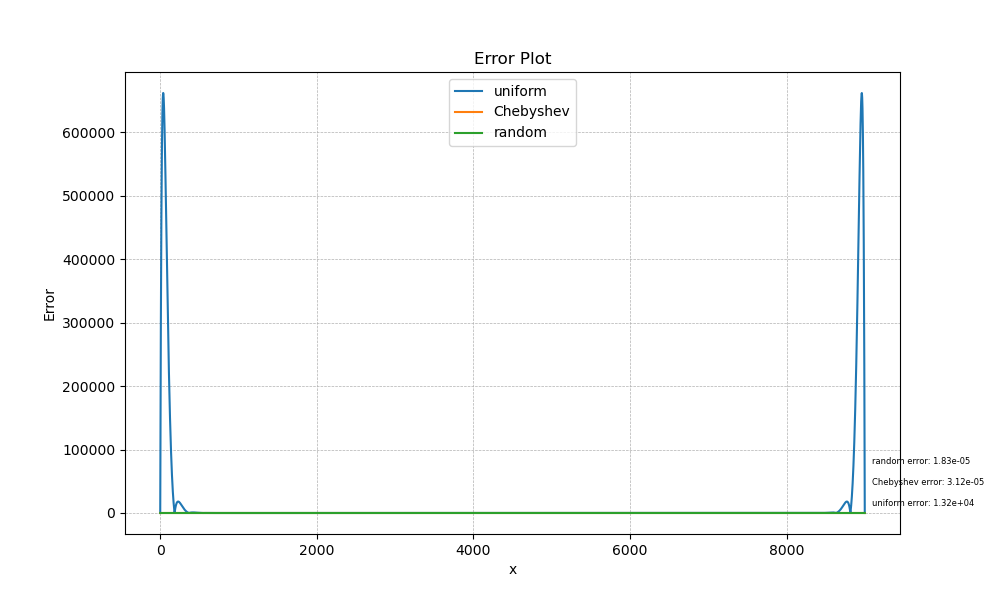
\includegraphics[width=0.75\textwidth]{prob1/contrast_error.png}
    \label{fig:contrast}
\end{figure}
\clearpage

\section{Least Square}
a,b为输入参数区间,目标函数形如$c \cdot \sin(d \cdot x) + e \cdot \cos(f \cdot x)$,参数n作为采样点的个数,参数m作为实验点的个数。全部使用切比雪夫正交多项式作为基函数以提高方法稳定性。
\subsection{Global Fitting}
在./data/prob2/prob2.21/prompts.json中可以看到未加扰动的原始输入,误差与函数对比由\hyperref[Fig:2.1,2.2]{Fig2.1}所示
\begin{figure}[H]
    \centering
    \includegraphics[width=0.8\textwidth]{prob2/fig212.png}
    \label{fig:2.1,2.2}
\end{figure}
此时误差处于可控范围内有两个原因,首先我们拟合的最高次数选的大,而且不过大,所以他有了足够又不过多的伸缩许可,其次所有原始输入均未引入扰动。
\par
为了测试野点对于二范数拟合的干扰程度,我们引入两种野点,第一种是全部点集在进入目标函数法则后都加入微小扰动,第二种是只引入少部分点但是扰动幅度大,这两种测试分别在代码的./data/prob2/prob2.21及.../prob2.22存有详细的原始输入信息及测试结果。\hyperref[fig:2.21,2.22]{Fig.2.3, Fig.2.4 }是两种干扰实施后的函数值对比.
\begin{figure}[H]
    \centering
    \includegraphics[width=0.67\textwidth]{prob2/fjg235.png}
    \label{fig:2.21,2.22}
\end{figure}
\clearpage
当引入少点数大扰动时,二范数的低抗噪性展露无遗。为了达到最小的最大误差,这种方法不可避免的存在着这样的局限。
\subsection{Local Fitting}
我们一直追求采样点与最高次数的独立性,能够解决这个依赖关系的只有“分段低次”。我们考虑段数为2,4,8下拟合情况,其中每个段数遍历最高次数[1,2,3,4]。同样,我绘制了很多详尽的图像,对每一种情况都进行了绘制,每一张图片都包含扰动点位置、gt位置、第k端的误差、目标函数走势、拟合函数走势...,均保存在./data/prob3/。
为了更好的说明分段的优越性,我们以拟合最高次数来区别每一个图像,因此有四个图像分别对应了所有分段情况下的一次拟合(线性拟合)、二次拟合、三次拟合以及四次拟合,如\hyperref[fig:3-1,3-2]{Fig:3-1,3-2} \hyperref[fig:3-3,3-4]{Fig:3-3,3-4.}
\begin{figure}[H]
    \centering
    \includegraphics[width=0.9\textwidth]{prob3/fig311.png}
    \label{fig:3-1,3-2}
\end{figure}
\begin{figure}[H]
    \centering
    \includegraphics[width=0.9\textwidth]{prob3/fig322.png}
    \label{fig:3-3,3-4}
\end{figure}
\clearpage
当引入扰动时,分段多次数小抗噪性略强,拟合度略高,如\hyperref[fig:3-5]{Fig.3-5}所示,从这里我们也可以看出分段的优势,减少了龙格的冗余权衡,用最简单的办法拟合最短的区域是非常好的想法。
\begin{figure}[H]
    \centering
    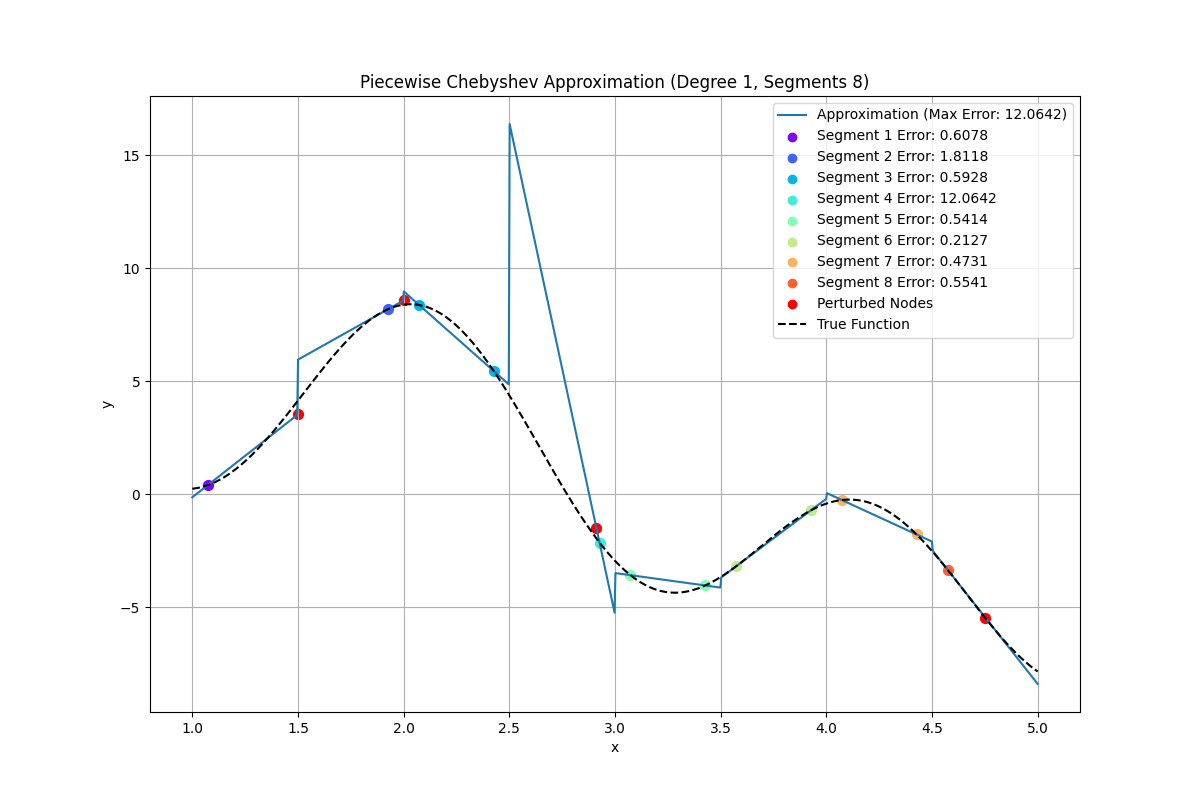
\includegraphics[width=0.9\textwidth]{prob3/new_prob3.2/piecewise_chebyshev_degree_1_segments_8.png}
    \caption*{Fig.3.5 degree:1,segments:8}
    \label{fig:3-5}
\end{figure}
另,我绘制了所有情况下扰动后的详细图如\hyperref[fig:3-5]{Fig.3-5}于./data/prob3/new\_prob3.2/,但是次数高了,加上扰动的存在,还是容易出现龙格效应,如\hyperref[fig:3-6]{Fig.3-6}所示
\begin{figure}[H]
    \centering
    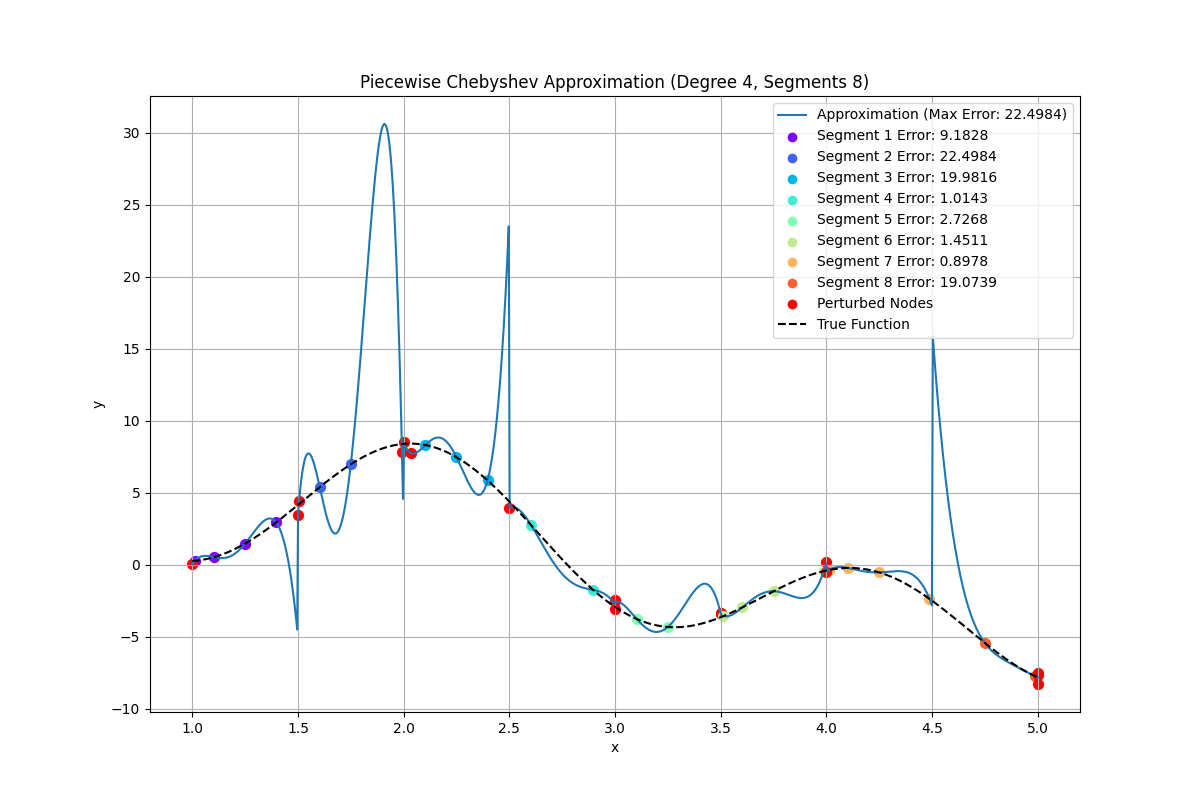
\includegraphics[width=0.75\textwidth]{prob3/new_prob3.2/piecewise_chebyshev_degree_4_segments_8.png}
    \caption*{Fig.3.6 degree:4,segments:8}
    \label{fig:3-6}
\end{figure}
\end{document}
